\documentclass[11pt]{article}
\usepackage[margin=2.6cm]{geometry}
\usepackage[spanish]{babel}
\usepackage[T1]{fontenc}
\usepackage{xcolor}
\usepackage{tikz}
\usetikzlibrary{calc}
% Comandos compartidos entre slides.tex y handout.tex
\usepackage{amsmath,amssymb}
\usepackage{siunitx}
\usepackage{booktabs}
\sisetup{per-mode=symbol}

\newcommand{\kB}{k_B}
\newcommand{\DG}{\Delta G}
\newcommand{\DGd}{\Delta G^{\ddagger}}
\newcommand{\Feq}{F_{\text{eq}}}
\newcommand{\peq}{p_{\text{eq}}}
\newcommand{\bhat}{\hat{F}}

% paleta sobria compartida (mismos tonos que el diagrama TikZ)
\definecolor{miazul}{RGB}{31,79,121}
\definecolor{minaranja}{RGB}{204,102,0}
\definecolor{migris}{RGB}{90,90,90}

% pie de figura compacto -- reutilizado en slides.tex y handout.tex
\newcommand{\Pie}[1]{%
  \vspace{0.4em}
  \begin{center}
  \begin{minipage}{0.82\textwidth}
    \centering{\scriptsize\color{migris}\itshape #1}
  \end{minipage}
  \end{center}%
}

\graphicspath{{../assets/}{figs/}}
% Diagrama de 3 paneles: paisaje real -> sesgo acumulado -> efecto neto plano
% Idea: el sesgo bien-templado converge a un "molde negativo" de F(s).
% Uso: \MoldeNegativoFigure[<scale>]
\newcommand{\MoldeNegativoFigure}[1][1]{%
\begin{tikzpicture}[scale=#1, every node/.style={font=\small}]

  % ---------- Panel 1: F(s) ----------
  \begin{scope}[xshift=0cm]
    \draw[->] (-0.3,0) -- (5.3,0) node[right] {\scriptsize $s$};
    \draw[->] (0,-0.3) -- (0,3.3) node[above] {\scriptsize $F(s)$};
    \draw[thick, blue!55!black, smooth, tension=0.85] plot coordinates {
      (0,2.6) (0.6,1.6) (1.1,0.35) (1.7,1.3) (2.3,2.9) (3.0,1.3) (3.6,0.85) (4.2,1.7) (4.8,2.7)
    };
    \node at (1.1,-0.6) {\scriptsize $A$};
    \node at (3.6,-0.6) {\scriptsize $B$};
    \node at (2.3,3.15) {\scriptsize barrera};
    \node[align=center] at (2.4,-1.15) {\footnotesize\bfseries Paisaje real};
  \end{scope}

  \draw[->, thick] (5.55,1.5) -- (6.35,1.5);

  % ---------- Panel 2: V(s,t) creciendo con el tiempo ----------
  \begin{scope}[xshift=6.7cm]
    \draw[->] (-0.3,0) -- (5.3,0) node[right] {\scriptsize $s$};
    \draw[->] (0,-0.3) -- (0,3.3) node[above] {\scriptsize $V(s,t)$};
    % fondo tenue: forma de -F(s), de referencia
    \draw[gray!35, smooth, tension=0.85] plot coordinates {
      (0,0.4) (0.6,1.4) (1.1,2.65) (1.7,1.7) (2.3,0.1) (3.0,1.7) (3.6,2.15) (4.2,1.3) (4.8,0.3)
    };
    % t1 (mas tenue, mas bajo)
    \draw[orange!40, smooth, tension=0.85] plot coordinates {
      (0.65,0) (1.1,0.85) (1.55,0) (3.25,0) (3.6,0.5) (3.95,0)
    };
    % t2 (medio)
    \draw[orange!70, smooth, tension=0.85] plot coordinates {
      (0.55,0) (1.1,1.65) (1.65,0) (3.15,0) (3.6,1.0) (4.05,0)
    };
    % t3 (mas oscuro, mas alto -- ya casi rellena los pozos de F(s))
    \draw[orange!95!black, thick, smooth, tension=0.85] plot coordinates {
      (0.45,0) (1.1,2.45) (1.75,0) (3.05,0) (3.6,1.55) (4.15,0)
    };
    \node[anchor=south west, align=left, font=\scriptsize] at (0.1,2.85) {$t_1 < t_2 < t_3$};
    \node[align=center] at (2.4,-1.15) {\footnotesize\bfseries Sesgo acumulado};
  \end{scope}

  \draw[->, thick] (12.35,1.5) -- (13.15,1.5);
  \node[align=center, font=\scriptsize] at (12.75,1.85) {$F+V$};

  % ---------- Panel 3: F(s)+V(s) practicamente plano ----------
  \begin{scope}[xshift=13.5cm]
    \draw[->] (-0.3,0) -- (5.3,0) node[right] {\scriptsize $s$};
    \draw[->] (0,-0.3) -- (0,3.3) node[above] {};
    \draw[blue!55!black, thick, smooth, tension=0.85] plot coordinates {
      (0,1.55) (0.8,1.48) (1.6,1.62) (2.4,1.5) (3.2,1.6) (4.0,1.48) (4.8,1.55)
    };
    \node[align=center] at (2.4,-1.15) {\footnotesize\bfseries Efecto neto};
    \node[align=center, font=\scriptsize] at (2.4,0.55) {el sistema difunde libremente};
  \end{scope}

\end{tikzpicture}%
}

\usepackage{graphicx}
\usepackage[colorlinks=true,linkcolor=miazul,citecolor=miazul,urlcolor=miazul]{hyperref}
\usepackage{enumitem}
\usepackage{tcolorbox}
\tcbuselibrary{skins,breakable}

\newtcolorbox{resultado}[1][]{colback=miazul!5,colframe=miazul,fonttitle=\bfseries,title={#1},breakable}
\newtcolorbox{aviso}[1][]{colback=minaranja!6,colframe=minaranja,fonttitle=\bfseries,title={#1},breakable}

\title{\textbf{Inventando la metadinámica}\\[0.3em]\large Derivaciones completas de respaldo}
\author{Metodología de Fernández-Quintero \emph{et al.} (2022) — Front. Immunol. \textbf{13}:953917}
\date{31 de agosto de 2026}

\begin{document}
\maketitle
\vspace{-1em}
\begin{center}
\small\color{migris}
Documento de respaldo para la charla \textit{Inventando la metadinámica}. Cubre las derivaciones completas del pipeline entero —problema, metadinámica \textit{well-tempered} y su precio, MD sembrada, tICA, MSM—, la munición de defensa/ataque, y un anexo reproducible del protocolo en PLUMED2/GROMACS/AMBER. El formulario de una página para la sesión de preguntas es un documento aparte (\texttt{formulario.pdf}).
\end{center}
\vspace{1em}

\tableofcontents

% ===================================================================
\section{El sistema}

\subsection{Un sistema modelo minimalista}
Los peces cartilaginosos son los organismos vivos \textbf{filogenéticamente más antiguos} con un sistema inmune adaptativo basado en inmunoglobulinas. Su anticuerpo, el \textbf{IgNAR}, es de cadena pesada únicamente —con origen evolutivo \emph{independiente} del de los VHH de camélidos, no una variante de ellos. Como el resto de los dominios de unión de cadena única (sdAbs), es pequeño ($\sim$12--15 kDa), muy estable, y accede a epítopos ``crípticos'' inaccesibles para un IgG convencional. El VNAR lleva esa lógica al extremo.

\begin{center}
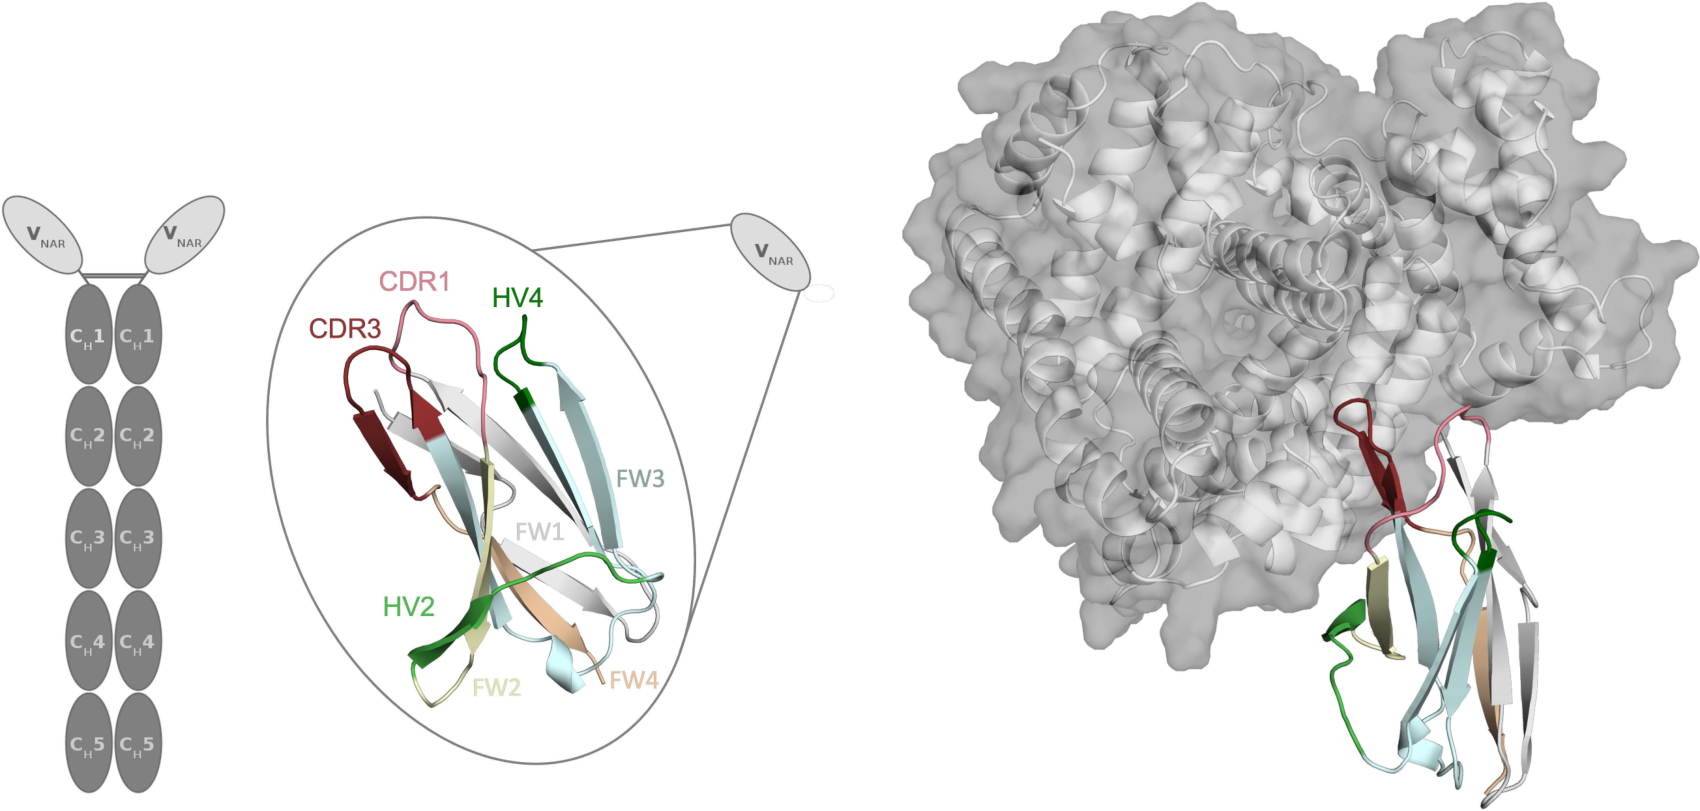
\includegraphics[width=0.72\textwidth]{fig1-vnar-estructura.png}
\Pie{Fig. 1 del paper: (A) esquema del IgNAR --- homodímero, 5 dominios constantes + 1 variable por cadena. (B) dominio VNAR aislado con CDR1/CDR3/HV2/HV4. (C) VNAR en complejo con HSA.}
\end{center}

\subsection{El dominio de unión más pequeño que existe}
\begin{center}
\begin{tabular}{lccc}
\toprule
 & Fv convencional & VHH (nanobody) & VNAR \\
\midrule
Cadenas en el paratopo & VH + VL & VH sola & VNAR sola \\
Nº de CDRs & 6 & 3 & \textbf{2} \\
\bottomrule
\end{tabular}
\end{center}
La CDR2 \textbf{no existe}: faltan las hebras $\beta$ C$'$/C$''$ que la sostienen en un plegamiento IgV típico. La compensación son \textbf{HV2} (cinturón lateral) y \textbf{HV4} (superior), regiones que en un anticuerpo convencional no son paratópicas. Consecuencia mecánica que se retoma en la \S\ref{sec:precio}: cualquier método que solo sesgue CDR1/CDR3 deja a HV2/HV4 fuera del muestreo mejorado.

\subsection{E06, el anticuerpo parental}
E06 fue aislado de una mielga inmunizada (\textit{Squalus acanthias}) y une HSA —también suero humano, de ratón y de rata— con alta afinidad. Existen cristales de dos miembros de la serie: \textbf{4HGK} (E06+HSA, 3.04 \r{A}) y \textbf{4HGM} (huE06 v1.1+HSA, 2.3 \r{A}).
\begin{quote}
\itshape ``E06 interacts with HSA in an atypical mode that utilizes extensive \textbf{framework} contacts in addition to complementarity-determining regions.''
\end{quote}
\begin{flushright}\small --- Kovalenko, Olland, Piche-Nicholas \textit{et al.}, \textit{J. Biol. Chem.} \textbf{288}:17408 (2013)\end{flushright}
Este es el paper de Pfizer que aisló y cristalizó E06/huE06 --- la referencia experimental que Fernández-Quintero \textit{et al.} reexaminan computacionalmente.

\subsection{Humanizar: tocar el framework, no las CDRs}
\begin{center}
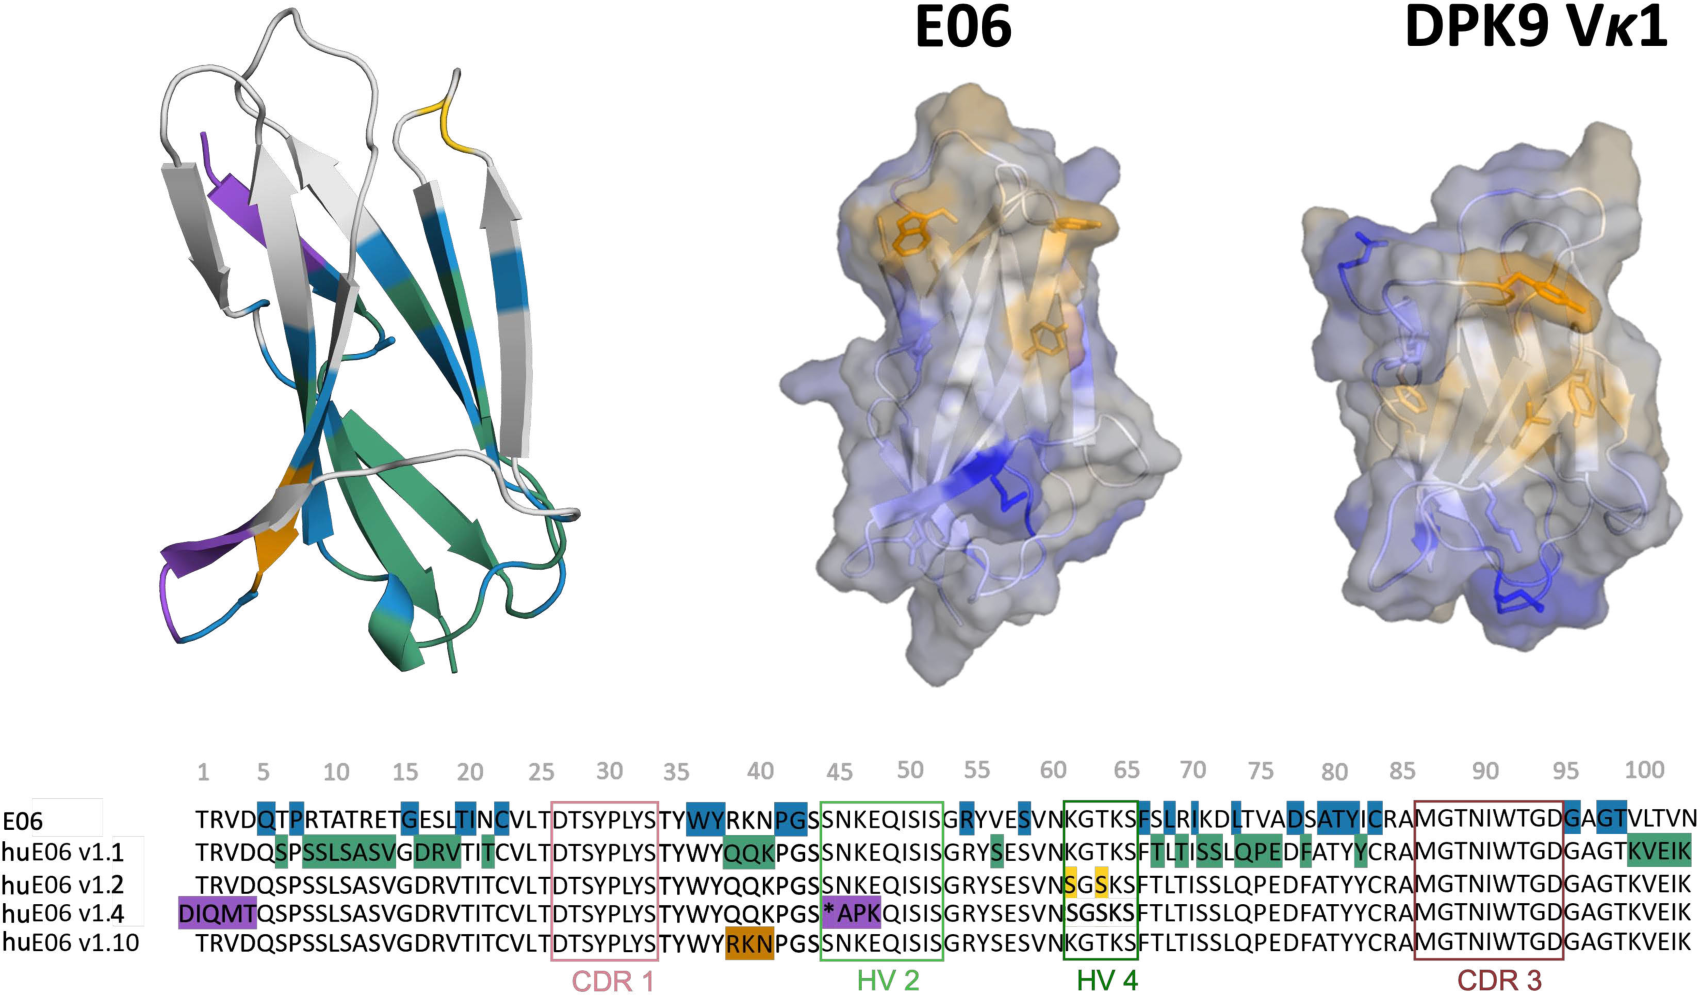
\includegraphics[width=0.68\textwidth]{fig2-alineamiento-hidrofobicidad.png}
\Pie{Fig. 2 del paper: (A) azul = idéntico a DPK9; verde/amarillo/morado = mutaciones de v1.1/v1.2/v1.4; naranja = motivo \texttt{RKN} revertido en v1.10. (B) hidrofobicidad de superficie (escala Wimley--White).}
\end{center}
Más del \textbf{60\%} de los residuos \emph{no}-CDR se convirtieron a los de la germinal humana \textbf{DPK9} (V$\kappa$1), en la cadena E06 $\to$ v1.1 $\to$ v1.2 $\to$ v1.4. La variante \textbf{v1.10} revierte el motivo \texttt{RKN} como control interno de reversión. DPK9 es cadena \emph{ligera}: en un Fab tiene una cara hidrofóbica de apareamiento con VH que, en el VNAR (que vive solo, sin pareja), queda expuesta al solvente.

\subsection{La paradoja que motiva el estudio}
\begin{quote}
\itshape ``The huE06 v1.1 molecule retained \textbf{all but one} amino acid residue involved in the binding site for HSA.''
\end{quote}
\begin{flushright}\small --- Kovalenko \textit{et al.} (2013)\end{flushright}
Casi el mismo sitio de unión, \'atomo por \'atomo —y sin embargo la afinidad y especificidad cambiaron. Si la estructura estática apenas varió, \textbf{¿qué cambió?} Esa pregunta es la que motiva mirar el \emph{ensemble} en solución en vez de una única conformación cristalográfica.

\subsection{Selección conformacional}
Bajo \textbf{selección conformacional}, el ligando captura un confórmero \emph{ya poblado}: lo que determina la afinidad es la población del estado competente \emph{antes} de que el antígeno llegue. Bajo \textbf{ajuste inducido}, en cambio, es el ligando quien moldea la conformación al unirse, y el estado apo no predice directamente la afinidad.
\begin{resultado}[Por qué este marco importa]
Bajo selección conformacional, ``¿cambió la humanización?'' se traduce en una pregunta computacionalmente precisa: \textbf{¿cambió la población del estado competente en ausencia de antígeno?} Ese es exactamente el número que el resto de este documento se ocupa de medir.
\end{resultado}

\subsection{El presupuesto computacional}
\begin{center}
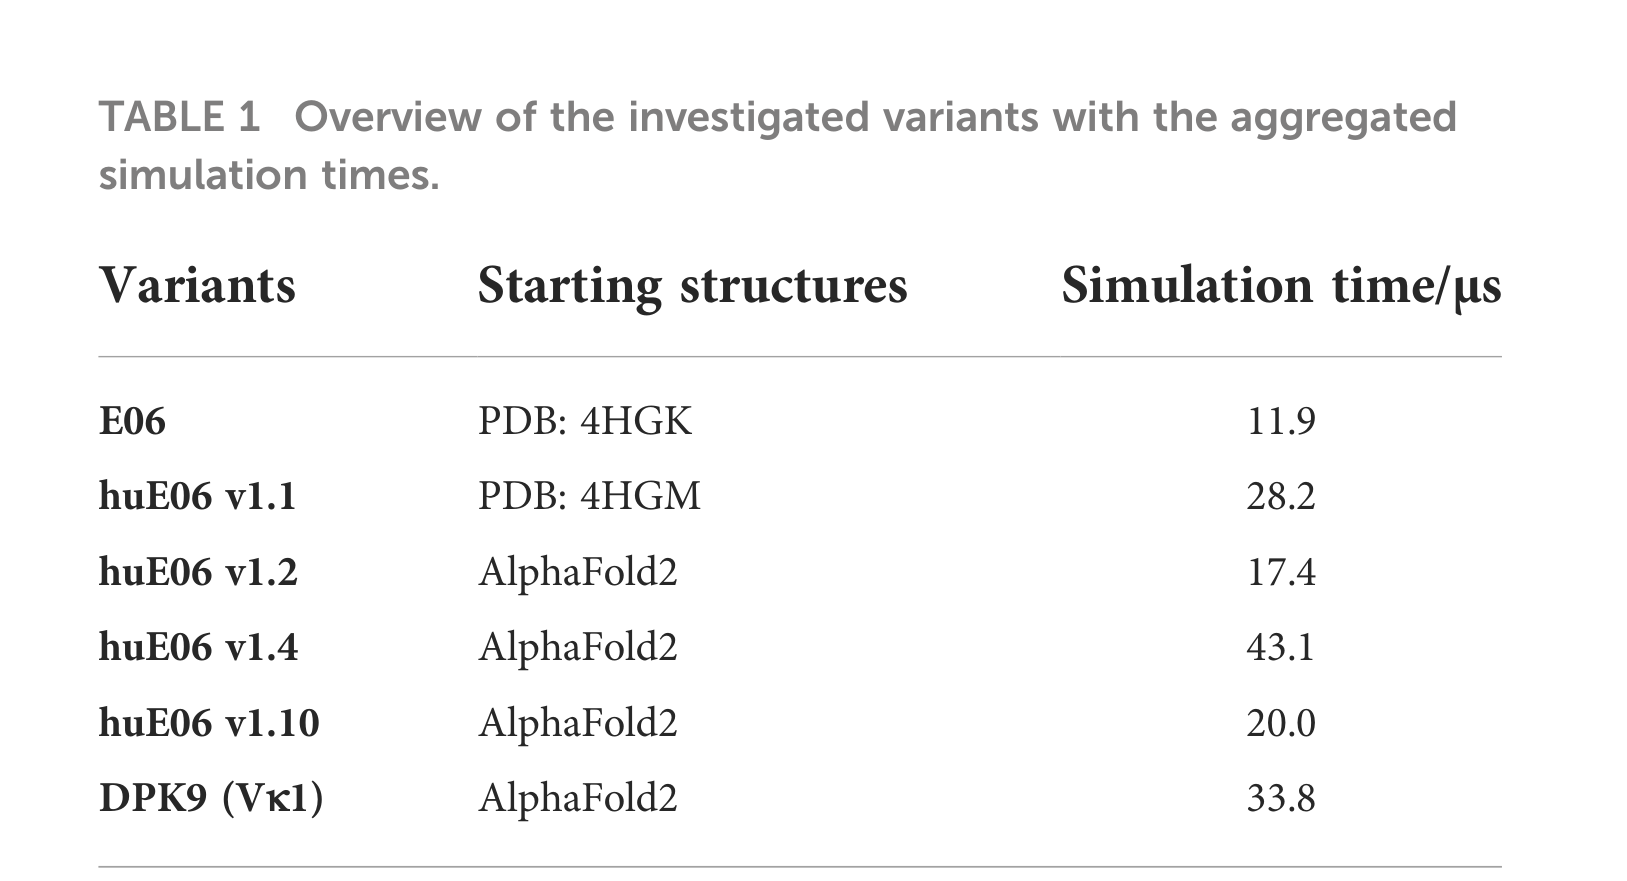
\includegraphics[width=0.55\textwidth]{tabla1-tiempos.png}
\Pie{Tabla 1 del paper. E06 y huE06 v1.1: estructuras de rayos X. El resto: modelos AlphaFold2.}
\end{center}
El tiempo agregado por sistema va de 11.9 a 43.1 $\mu$s —una asimetría que se retoma como posible confusión muestreo/observable fuera del alcance de este documento (ver notas de la Clase 1).

% ===================================================================
\section{El problema: poblaciones, barreras, y por qué la MD sola no basta}

\subsection{Poblaciones de equilibrio}

En el ensemble canónico, $p(\mathbf{r}) = e^{-\beta U(\mathbf{r})}/Z$ con $\beta \equiv 1/RT$. Proyectando sobre una variable colectiva (CV) $s=\xi(\mathbf{r})$ vía marginalización,
$$p(s) = \big\langle \delta(\xi(\mathbf{r})-s) \big\rangle,$$
se define el \emph{potential of mean force} $F(s) \equiv -RT\ln p(s) + C$. Para dos macroestados $A,B$, con $G_A \equiv -RT\ln Z_A$,
$$\frac{P_A}{P_B} = e^{-(G_A-G_B)/RT} \qquad\Longleftrightarrow\qquad \DG_{AB} = -RT\ln\frac{P_A}{P_B}.$$
A 300 K, $RT = 8.314\times300 = \SI{2494}{\joule\per\mole}\approx \SI{2.5}{\kilo\joule\per\mole}$: un factor $e$ en población cuesta 2.5 kJ/mol; un factor 10 cuesta $RT\ln10\approx\SI{5.7}{\kilo\joule\per\mole}$.

\textbf{Aplicación:} con $P=0.92$ (estado competente de E06), $\DG = -RT\ln(0.92/0.08) = -6.1$ kJ/mol. Con $P=0.16$ (huE06 v1.1), $\DG' = +4.1$ kJ/mol. El efecto completo:
$$\DG_{AB} = 4.1-(-6.1) \approx \mathbf{10.2\ kJ/mol} \approx 2.4\ \text{kcal/mol}.$$
Esa cifra —modesta en unidades de $RT$ (4$RT$)— es comparable a la incertidumbre típica de un campo de fuerza en energías conformacionales de lazos acumuladas sobre 10--15 residuos.

\begin{center}
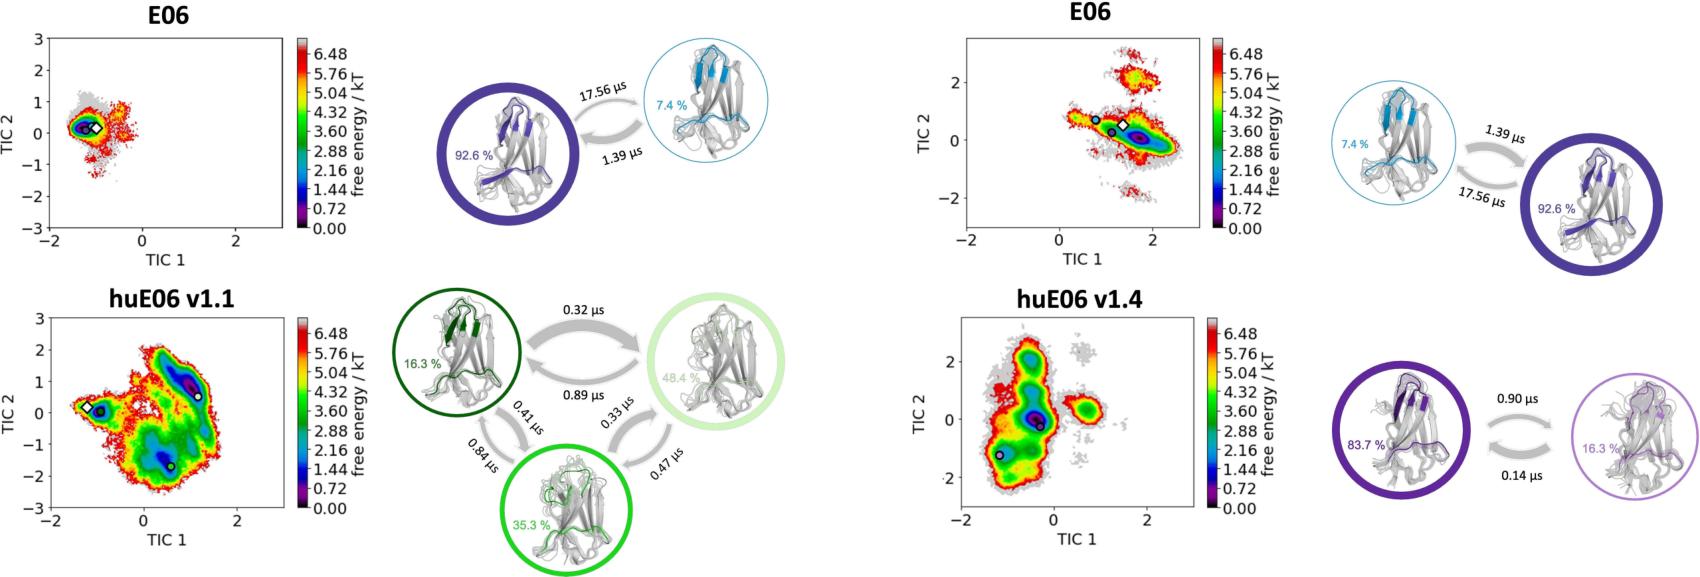
\includegraphics[width=0.9\textwidth]{fig4-msm-poblaciones.png}
\Pie{Fig. 4 del paper: paisajes con probabilidades de macroestado y tiempos de transición, parent E06 vs. huE06 v1.1 (izq.) y vs. huE06 v1.4 (der.). Rombo blanco = estructura cristalográfica.}
\end{center}
E06: \textbf{92.6\%}/7.4\% $\to$ huE06 v1.1: 16.3\%/48.4\%/35.3\%.

\subsection{Por qué las barreras importan}

Por teoría del estado de transición, con coeficiente de transmisión $\kappa\le1$,
$$k = \kappa\,\frac{\kB T}{h}\,e^{-\DGd/RT}, \qquad \tau = 1/k, \qquad \frac{\kB T}{h}\Big|_{300\text{K}} = 6.25\times10^{12}\ \text{s}^{-1}.$$
Para $\DGd=40$ kJ/mol: $\beta\DGd=16.04$, $k_{\text{TST}}=6.75\times10^5\ \text{s}^{-1}$, $\tau\approx1.5\ \mu$s (cota superior con $\kappa=1$; con $\kappa\sim10^{-2}$ realista, $\tau\sim150\ \mu$s). El número esperado de cruces en 100 ns es $\langle n\rangle = k\,t \approx 7\times10^{-2}$ (cota superior): \textbf{no ocurre}.

Invirtiendo para $\langle n\rangle\approx1$ en 100 ns con $\kappa=10^{-2}$: $\DGd\approx22$ kJ/mol. \textbf{100 ns de MD compran barreras de hasta $\sim$22 kJ/mol}, y las transiciones de lazos CDR viven en 25--45 kJ/mol.

\subsection{Y si el muestreo está mal repartido}
Los números anteriores presuponen que $P$ se midió correctamente. Si se agrupan trayectorias de distintas cuencas $i$ con pesos $w_i\ne\pi_i$ (el peso de Boltzmann verdadero), la ``energía libre'' resultante es
$$\hat F(s) = F(s) - RT\ln\frac{w_i}{\pi_i}, \qquad s\in\text{cuenca } i.$$
El error \textbf{no depende de $s$} dentro de una cuenca (la \emph{forma} de cada pozo sale correcta), pero \textbf{sí depende de $i$} (las \emph{profundidades relativas} —es decir, las poblaciones— salen mal), y \textbf{no decrece con más muestreo}: es sesgo sistemático, no ruido estadístico. Este resultado es el que obliga a que, más adelante en el pipeline, ninguna etapa pueda saltarse la reponderación hacia $\pi_i$ (fuera del alcance de este documento).

\begin{aviso}[Distinción crítica: $\DG$ frente a $\DGd$]
Son cantidades \emph{independientes} —$\DG$ entre mínimos (controla poblaciones), $\DGd$ entre mínimo y cima (controla velocidad). Por balance detallado, escribiendo las tasas desde el mismo estado de transición y dividiendo (el término $F(s^\ddagger)$ se cancela):
$$\frac{k_{A\to B}}{k_{B\to A}} = e^{-\DG/RT} = \frac{P_B}{P_A}.$$
\textbf{La barrera no aparece en el cociente.} Controla cuánto tarda el sistema en equilibrar, no dónde está el equilibrio. Este sistema combina pozos someros ($\DG\approx6$ kJ/mol, $2.4RT$) con muros altos ($\DGd\approx25$--45 kJ/mol, $10$--$18RT$): alta precisión sobre un número pequeño, en un sistema que se niega a equilibrarse solo.
\end{aviso}

% ===================================================================
\section{Inventar la metadinámica}

\subsection{Por qué no basta con subir la temperatura}
Duplicar $T$ (300$\to$600 K) acelera $\sim$6000$\times$ una barrera de 40 kJ/mol —funciona. Pero: (i) acelera \emph{todo} el sistema indiscriminadamente, no solo el grado de libertad de interés; (ii) reponderar de vuelta a 300 K requiere pesos $e^{-\Delta\beta\,U(\mathbf{r})}$ con $U$ extensiva ($\sim10^5$ kJ/mol, fluctuaciones $\sim\sqrt{N}$) —varianza inmanejable; (iii) no se puede apuntar a una CV concreta. Ésta es la base de REMD, un método legítimo pero distinto, y con la ventaja de no requerir elegir CVs de antemano.

\subsection{Un sesgo sobre la CV se suma exactamente al paisaje}
Sea $U_V(\mathbf{r}) = U(\mathbf{r}) + V(\xi(\mathbf{r}))$. Marginalizando y usando que, bajo el filtro $\delta(\xi(\mathbf{r})-s)$, $V(\xi(\mathbf{r}))=V(s)$ es constante y sale de la integral (mientras $U(\mathbf{r})$ varía dentro del mismo conjunto de nivel y no sale):
$$p_V(s) \propto \peq(s)\,e^{-\beta V(s)} \qquad\Longrightarrow\qquad \boxed{F_V(s) = F(s) + V(s)}.$$
El sesgo que aplana el paisaje por completo es $V^{\text{ideal}}=-F$ —pero calcularlo requiere conocer $F$: el huevo y la gallina que la metadinámica resuelve.

\subsection{Sesgo adaptativo y el problema de la convergencia}
Esto ocurre \textbf{en tiempo real, dentro de la propia corrida} --- no es un post-proceso sobre una trayectoria ya generada. PLUMED está acoplado a GROMACS: en \emph{cada} paso de integración (2 fs), se calcula la fuerza a partir de $U(\mathbf r)+V(\xi(\mathbf r),t)$ con el $V$ acumulado \emph{hasta ese instante}, y esa fuerza mueve los átomos igual que cualquier otra fuerza física. Cada $\tau_G$ pasos, además, se agrega una gaussiana nueva al registro de $V$, centrada en la posición actual del sistema:
$$V(s,t) = \sum_{t'<t} W\,e^{-(s-\xi(\mathbf{r}(t')))^2/2\sigma^2}.$$
La tasa de deposición sigue $\partial_tV(s,t) \propto p_V(s,t) \propto e^{-\beta[F(s)+V(s,t)]}$: donde $F$ es bajo, el sistema visita más, deposita más rápido, y el paisaje se autorregula hacia $V\to-F+\text{const}$. \textbf{Pero la deposición nunca cesa} —con el paisaje plano, $\partial_tV$ es uniforme pero no cero, y el sistema escapa hacia regiones de energía absurdamente alta (\emph{overfilling}). Con los parámetros del paper (10 kJ/mol cada 2 ps, 1 $\mu$s), el sesgo total sin freno sería $5\times10^6$ kJ/mol —$125\,000$ veces la barrera de interés.

\subsection{Well-tempered: el freno}
La altura decae con el sesgo ya acumulado: $W(s,t)=W_0\,e^{-V(s,t)/\kB\Delta T}$. Imponiendo que la \emph{tasa} de deposición sea uniforme en $s$ (condición de convergencia de forma), y usando $\gamma\equiv(T+\Delta T)/T$:
$$\frac{T}{\Delta T}V(s) + F(s) + V(s) = \text{const} \quad\Longrightarrow\quad V(s)\cdot\frac{T+\Delta T}{\Delta T}=-F(s)+\text{const}$$
$$\Longrightarrow\quad \boxed{V(s)\xrightarrow[t\to\infty]{} -\frac{\gamma-1}{\gamma}F(s)}.$$
De aquí, sustituyendo en $F_V=F+V$ y en $p_V\propto e^{-\beta F_V}$:
$$F_V(s) = \frac{F(s)}{\gamma}, \qquad p_V(s) \propto \peq(s)^{1/\gamma}, \qquad F(s) = -\frac{\gamma}{\gamma-1}V(s).$$
Límites: $\gamma\to1 \Rightarrow V\to0$ (MD normal); $\gamma\to\infty \Rightarrow V\to-F$ (metadinámica estándar, no converge). $\gamma$ interpola entre ambos.

\begin{center}
\resizebox{\textwidth}{!}{\MoldeNegativoFigure[1]}
\end{center}

\begin{resultado}[Números del paper]
CVs: $\sin\psi,\cos\psi$ de CDR1 y CDR3 (torsiones de \emph{backbone}, vía \texttt{MATHEVAL}+\texttt{COMBINE} en PLUMED 2). $\gamma=10 \Rightarrow \Delta T=2700$ K (CV a 3000 K). Altura 10 kJ/mol, ancho 0.3 rad, cada 1000 pasos ($=$2 ps), 1 $\mu$s por sistema. Barrera efectiva: $40/\gamma=4$ kJ/mol $\Rightarrow$ $\tau\approx0.8$ ps, aceleración $\approx1.9\times10^6$ frente al valor sin sesgo.
\end{resultado}

% ===================================================================
\section{El precio}
\label{sec:precio}

\subsection{La cinética se comprime de forma no uniforme}
El factor de aceleración de una transición concreta es $\alpha = e^{\beta\DGd(\gamma-1)/\gamma}$ —\textbf{depende de la barrera}. Para dos transiciones $A,B$:
$$\frac{\tau_A^V}{\tau_B^V} = \left(\frac{\tau_A}{\tau_B}\right)^{1/\gamma}.$$
Ejemplo: una separación real de $23\,000\times$ queda, bajo $\gamma=10$, en $23\,000^{0.1}\approx2.7\times$ —cuatro órdenes de magnitud aplastados a un factor 3. \textbf{No es un efecto secundario: es el mecanismo.} (Existe un método para recuperar cinética real, \emph{infrequent metadynamics} de Tiwary \& Parrinello, PRL \textbf{111}:230602, 2013 —pero exige depositar sesgo muy espaciadamente, régimen opuesto al usado aquí, que persigue exploración, no cinética.)

\subsection{Las CVs son una elección mecánica, no solo estadística}
La fuerza de sesgo sobre el átomo $i$, por regla de la cadena:
$$\mathbf{f}_i^{\text{sesgo}} = -\frac{dV}{ds}\,\nabla_{\mathbf{r}_i}\xi(\mathbf{r}).$$
Si el átomo $i$ no participa en la definición de $\xi$ (p. ej., cualquier átomo de HV2, o cualquiera de las $\sim$29\,000 aguas), $\nabla_{\mathbf{r}_i}\xi=\mathbf{0}$ y la fuerza es \textbf{exactamente cero} —no decreciente con la distancia, sino nula por pertenencia. Con las CVs del paper ($\sim$27 torsiones $\psi$, $\sim$100 átomos), \textbf{$\sim$0.3\% del sistema recibe empuje}; el 99.7\% restante —incluida HV2— corre MD clásica pura durante todo el microsegundo.

\subsection{La jugada: tirar $F$ y la cinética, quedarse con las estructuras}
\begin{center}
\begin{tabular}{lcc}
\toprule
Producto & Estado & ¿Se usa? \\
\midrule
Energía libre $F(s)$ & sin convergencia verificada & no \\
Cinética & comprimida, no física & no \\
\textbf{Conjunto de estructuras} & diverso y útil & \textbf{sí} \\
\bottomrule
\end{tabular}
\end{center}
\begin{quote}
\small\itshape ``Being only used to generate initial conformations, the implementation of metadynamics can be simple and fast.''\\
\upshape --- Biswas, Lickert \& Stock, \textit{J. Phys. Chem. B} \textbf{122}:5508 (2018)
\end{quote}
Al usar la metadinámica \emph{solo} como generador de conformaciones, \textbf{la convergencia deja de ser un requisito} —no hace falta que converja, solo que haya recorrido sitios variados. Esto desactiva ambas facturas (energía libre mal proyectada, cinética destruida) simultáneamente. Lo que se hereda es el peso de siembra $w_i$ de cada cluster, que en general $w_i\ne\pi_i$ (el peso de Boltzmann verdadero) —el problema que la etapa siguiente del pipeline (MD sembrada + Markov State Model) está diseñada para reparar, y que queda fuera del alcance de este documento.

\vspace{1em}
\begin{aviso}[Lo que sobrevive de la factura de las CVs]
Tirar $F$ elimina la factura \emph{termodinámica} de elegir CVs, pero no la \emph{estructural}: un modelo posterior solo puede reponderar los estados que alguien visitó. Si un grado de libertad lento nunca se sesgó y nunca se pobló, ningún análisis posterior lo rescata.
\end{aviso}

% ===================================================================
\section{MD sembrada}

Las trayectorias de metadinámica se agrupan por \textbf{clustering jerárquico} (\textit{average linkage}, \texttt{cpptraj}) con un corte de \textbf{1.3 \r{A}}. Cada representante de cluster se equilibra y se simula \textbf{100 ns sin sesgo} (AMBER 20, \texttt{pmemd.cuda}). El paper reporta ``\textit{a large number of clusters}'' remitiendo a la Tabla 1 --- pero la Tabla 1 solo publica tiempo agregado, no el número de clusters. El número de clusters por variante fija $w_i$ sin que ninguna decisión explícita lo controle: emerge del corte de distancia fijo aplicado a paisajes con distinta dispersión.

% ===================================================================
\section{tICA: encontrar lo lento}

Con cientos de trayectorias de 100 ns en un espacio de muchas torsiones, hace falta una proyección a baja dimensión para visualizar el paisaje. La opción ingenua, \textbf{PCA}, maximiza \emph{varianza} --- pero un lazo puede bambolearse mucho sin ser el modo más \emph{lento}, que es el que separa estados metaestables. \textbf{tICA} resuelve el problema de autovalores generalizado
$$C(\tau)\,v = \lambda\,C(0)\,v,$$
donde $C(\tau)$ es la matriz de covarianza \textbf{desfasada} en el tiempo y $C(0)$ la instantánea. Los autovectores de mayor autovalor son las direcciones que menos se decorrelacionan al esperar un tiempo $\tau$: las más lentas del sistema.

El paper usa como \emph{features} las torsiones de \emph{backbone} de \textbf{CDR1, CDR3 y HV2}, con lag $\tau=10$ ns (PyEMMA 2). Aquí reaparece la asimetría del \S\ref{sec:precio}: \textbf{HV2 nunca fue una CV de metadinámica, pero sí es una \emph{feature} de tICA} --- se mide, aunque nunca se muestreó con sesgo.

% ===================================================================
\section{El Markov State Model}

\subsection{Qué estima}
Los 100 microestados se definen por k-means sobre las coordenadas tICA. Contando transiciones $i\to j$ a un lag $\tau=15$ ns (distinto del lag de tICA, 10 ns) se obtiene la matriz de conteos $C_{ij}(\tau)$, y normalizando, la \textbf{matriz de transición} $T(\tau)$. Todo lo que sigue sale de $T(\tau)$ por álgebra lineal:
$$\pi^\top T(\tau) = \pi^\top \quad\text{(población de equilibrio, autovector izquierdo de autovalor 1)}$$
$$t_i = -\frac{\tau}{\ln\lambda_i} \quad\text{(tiempos característicos, de los autovalores subdominantes)}$$
\textbf{PCCA+} (Röblitz \& Weber, \textit{Adv. Data Anal. Classif.} \textbf{7}:147, 2013) agrupa los microestados en macroestados usando el signo de los autovectores lentos de $T$.

\subsection{Por qué $\pi$ no depende de la siembra}
\begin{resultado}[El nodo que legitima todo el pipeline]
$\pi$ sale de las \textbf{tasas locales} $T_{ij}$, no de cuántas veces se visitó cada microestado. Sembrar más en una región mejora la \emph{precisión} con la que se estima $T_{ij}$ ahí --- no cambia su valor esperado, siempre que haya suficientes transiciones observadas para estimarlo. Esto es, formalmente, lo que resuelve el problema planteado en \S\ref{sec:precio}: $\hat F(s) = F(s) - RT\ln(w_i/\pi_i)$ --- el MSM reponde $w_i \to \pi_i$. Es la respuesta formal a la objeción ``pero la siembra estaba sesgada''.
\end{resultado}

\subsection{Validación}
El \textbf{test de Chapman--Kolmogorov} comprueba $T(n\tau) \approx [T(\tau)]^n$; si falla, el lag elegido es demasiado corto para que la dinámica sea markoviana a esa escala (Prinz \textit{et al.}, \textit{J. Chem. Phys.} \textbf{134}:174105, 2011 --- la referencia canónica del test aplicado a MSMs; el paper cita en su lugar dos referencias sobre la ecuación de Chapman--Kolmogorov en abstracto, no sobre el test de validación). \textbf{VAMP} (Wu \& Noé, \textit{J. Nonlinear Sci.} \textbf{30}:23, 2017) da un score variacional para elegir lag y \emph{features} óptimos. Y se exige la \textbf{fracción de estados conectados}, necesaria para que $\pi$ tenga sentido.

% ===================================================================
\section{Resultados}

\begin{center}
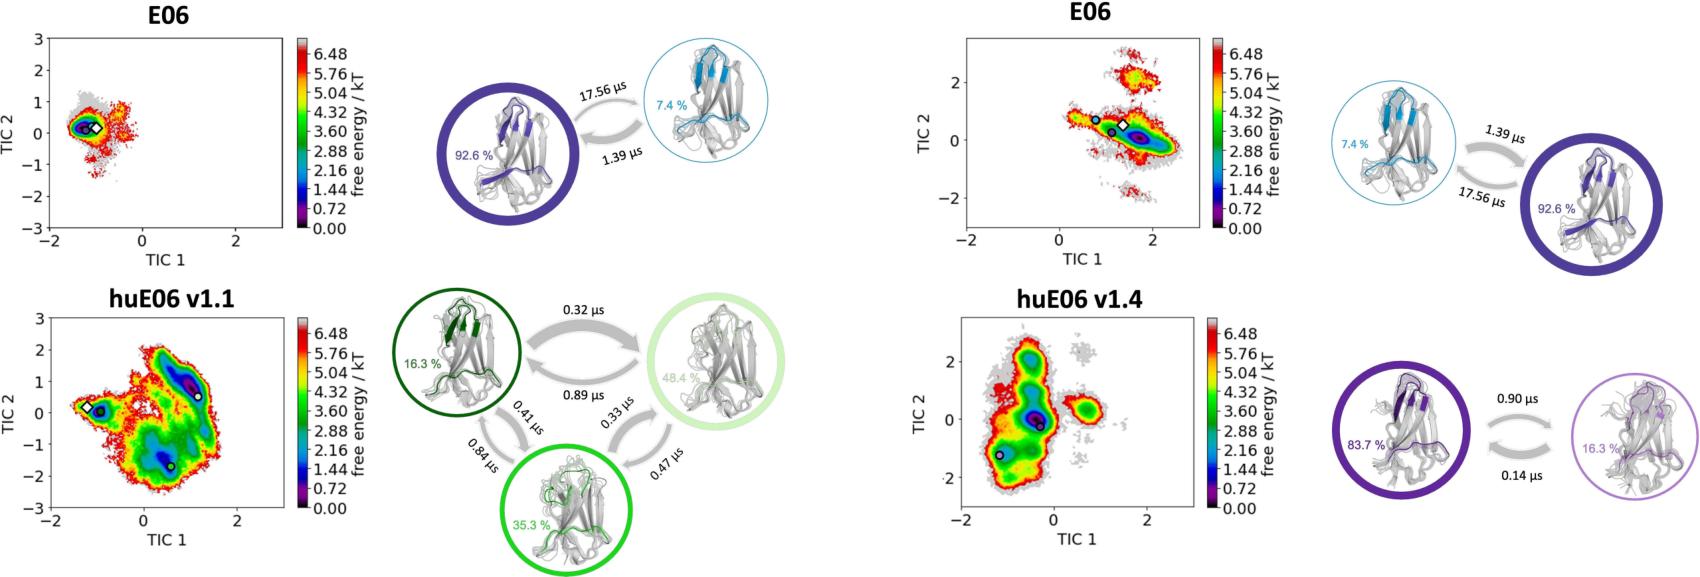
\includegraphics[width=0.92\textwidth]{fig4-msm-poblaciones.png}
\Pie{Fig. 4 del paper --- el resultado completo, construido por metadinámica $\to$ clustering $\to$ MD sembrada $\to$ tICA $\to$ MSM.}
\end{center}
E06: \textbf{92.6\%}/7.4\%. huE06 v1.1: 16.3\%/48.4\%/35.3\%. huE06 v1.4: 83.7\%/16.3\%.

\begin{center}
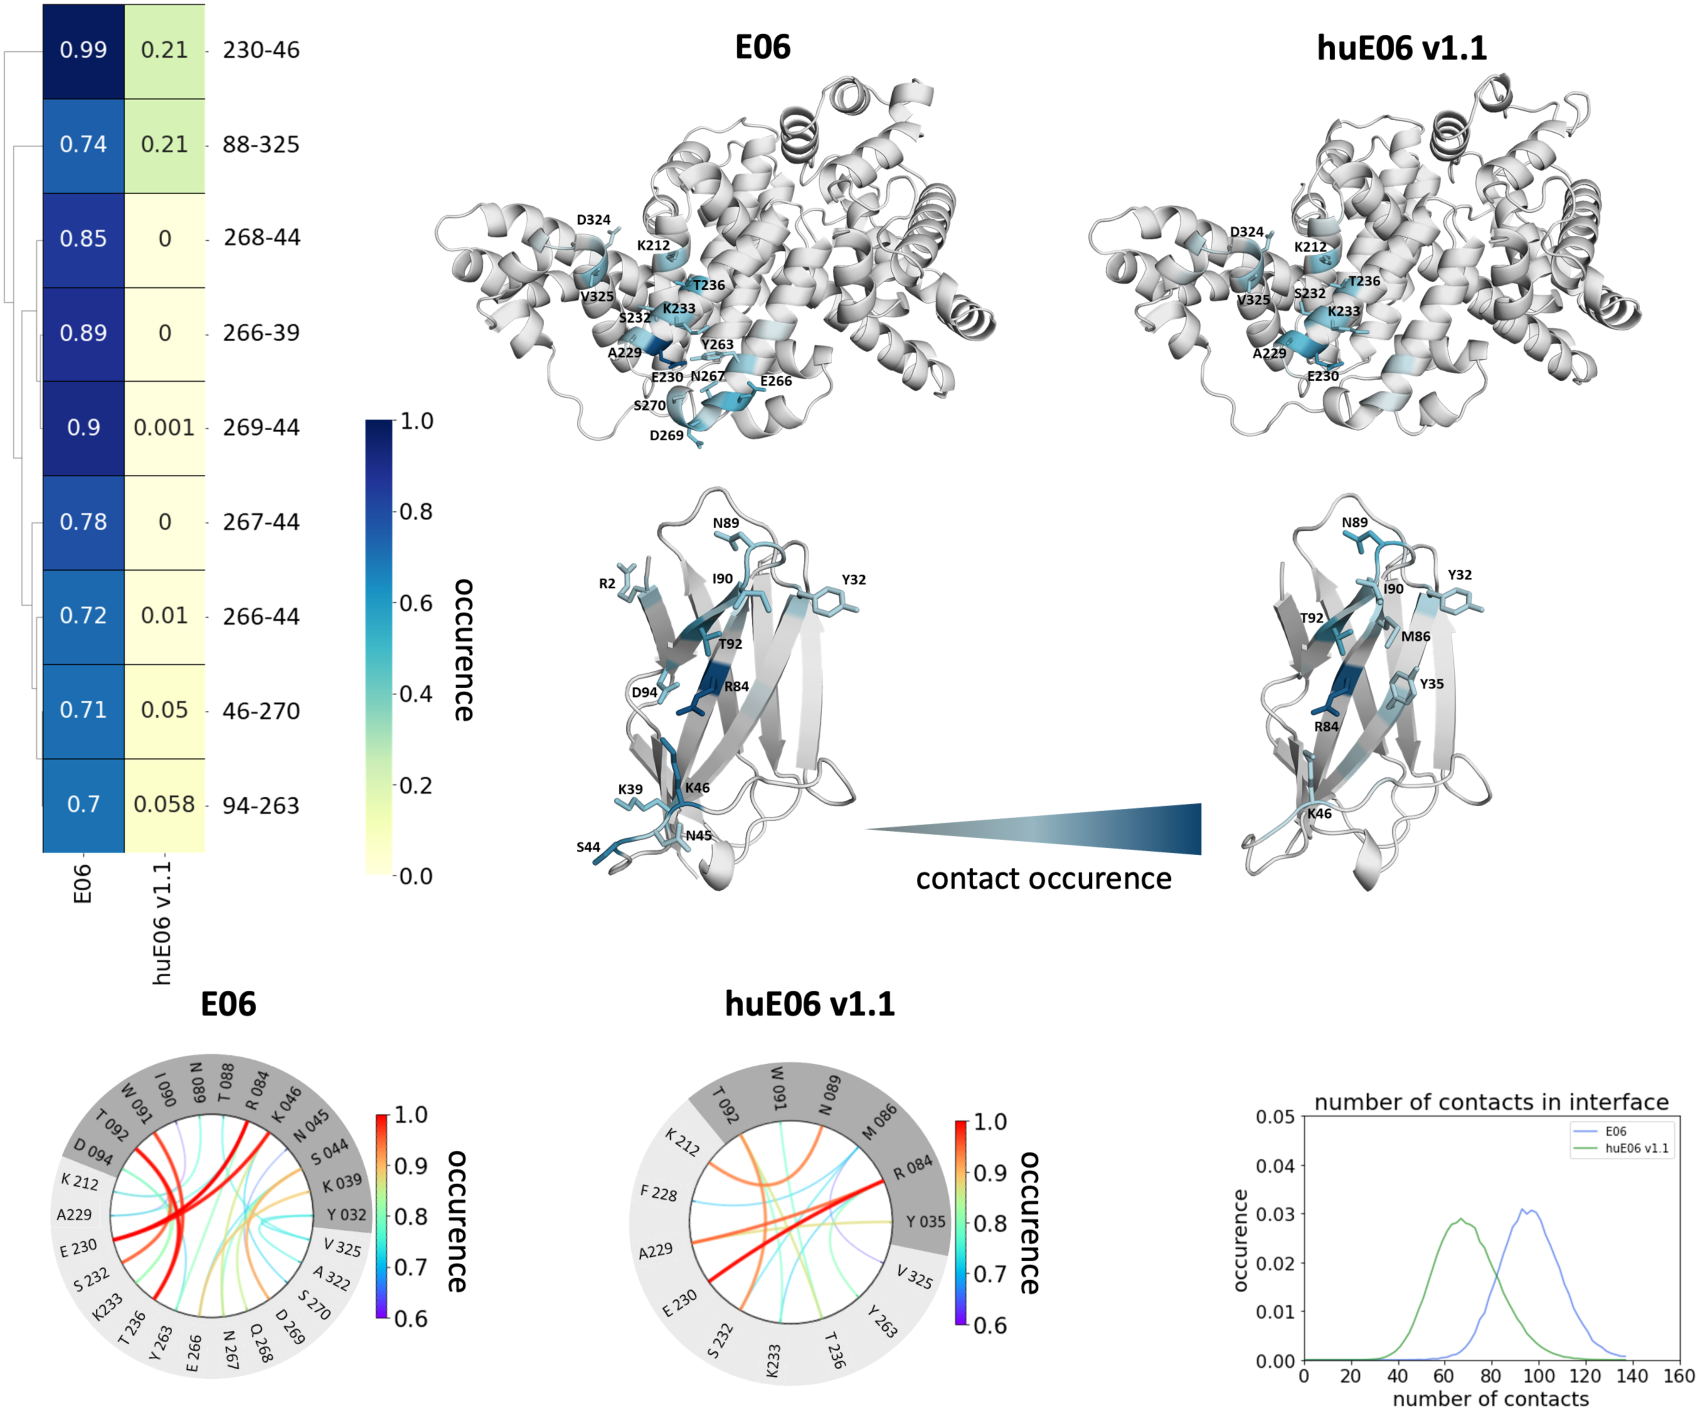
\includegraphics[width=0.62\textwidth]{fig5-contactos-hsa.png}
\Pie{Fig. 5 del paper: mapas de contacto E06--HSA vs. huE06 v1.1--HSA. La frecuencia de contacto cae de 0.7--0.99 a 0--0.21.}
\end{center}
El paper atribuye la pérdida de afinidad a ``\textit{missing interactions with the \textbf{HV2} loop and the framework}''.

% ===================================================================
\section{Munición: defensa}

El pipeline no es un protocolo \textit{ad hoc}: lleva $\sim$5 años rodando en el grupo Liedl. Genealogía parcial (citas según OpenAlex): CDR-H3 loop ensembles (\textit{Front. Immunol.} 2019, 96 citas), conformational selection en CDR-H3 (\textit{mAbs} 2019, 72), ensembles vs. clusters de rayos X (\textit{mAbs} 2020, 34), ensembles como paradigma de diseño (\textit{mAbs} 2021, 30), y --- la carta más fuerte --- \textbf{Nanobody Paratope Ensembles in Solution Characterized by MD Simulations and NMR} (\textit{IJMS} 2022, 19 citas), que valida el mismo método contra \textbf{RMN experimental} en un sistema hermano.

% ===================================================================
\section{Munición: ataque}

\subsection{Las críticas más fuertes}
\begin{center}
\small
\begin{tabular}{clc}
\toprule
 & Crítica & Severidad \\
\midrule
A1 & Muestreo confundido con el observable (11.9 vs.\ 43.1 $\mu$s) & alta \\
A2 & HV2 nunca sesgada, pero sostiene la conclusión biológica & alta \\
A3 & Ni una barra de error (\texttt{BayesianMSM} gratis en PyEMMA) & alta \\
A4 & Lag 15 ns vs.\ trayectorias de 100 ns ($\sim$6.7 lags/trayectoria) & media \\
A6 & ¿Fig.\ 3A reponderada por el MSM, o histograma crudo? & media \\
\bottomrule
\end{tabular}
\end{center}

\textbf{A1.} El corte de clustering fijo (1.3 \r{A}) hace que un sistema más flexible genere más clusters, más semillas, y más tiempo agregado: E06 (``rígido'') recibe 11.9 $\mu$s frente a los 43.1 $\mu$s de huE06 v1.4 (``flexible''), $3.6\times$ más. La entropía dihedral (KDE) y el área del espacio tICA crecen monótonamente con el número de frames, así que las comparaciones entre variantes no están desacopladas del muestreo que recibieron.

\textbf{A2 (versión mecánica).} Los átomos de HV2 no recibieron ni una sola fuerza de sesgo en todo el microsegundo de metadinámica (\S\ref{sec:precio}). Su muestreo es exactamente el de MD clásica sin sesgo --- que compra barreras de hasta $\sim$22 kJ/mol (\S2.2) --- y sin embargo entra en tICA y en el MSM, sosteniendo la conclusión de que la pérdida de afinidad se debe a HV2.

\textbf{A2 (las implicancias).} La estructura lógica exacta: (1) HV2 nunca fue CV, fuerza de sesgo cero sobre sus átomos; (2) HV2 sí es \textit{feature} de tICA y sí entra al MSM; (3) el paper atribuye la pérdida de afinidad a \textit{``missing interactions with the HV2 loop''} (Fig.\ 5, Discusión). Esto deja \textbf{dos lecturas indistinguibles con los datos publicados}: \textbf{(a)} el movimiento de HV2 es una respuesta correlacionada real, transmitida por física clásica cuando CDR1/CDR3 se reacomodan bajo sesgo --- legítima \emph{si} está bien muestreada; \textbf{(b)} es un artefacto de submuestreo --- ningún análisis posterior (tICA, MSM) puede reconstruir un cruce de barrera de HV2 que jamás se sesgó, por buena que sea la estadística sobre los datos que sí existen. El paper no ofrece ninguna forma de distinguir (a) de (b), y la conclusión mecanicista sobre por qué la humanización reduce la afinidad depende de que sea (a).

\begin{aviso}[Hallazgo propio: ¿cuadra la Fig.\ 4D?]
En los paneles A/C de la Fig.\ 4, el estado \textbf{dominante} de E06 (92.6\%) se dibuja en \textbf{morado oscuro}. En el panel D (huE06 v1.4), el morado oscuro corresponde al \textbf{83.7\%}, mientras que el texto identifica el estado competente de v1.4 con el \textbf{16\%}. Si el color codifica correspondencia estructural entre paneles --- y v1.4 no tiene cristal propio para anclar la asignación --- el análogo del estado dominante de E06 parecería ser el 83.7\%, no el 16.3\%. No se afirma como error confirmado: es una pregunta legítima para la sesión de preguntas.
\end{aviso}

\subsection{Alternativas no discutidas}
\begin{center}
\small
\begin{tabular}{lp{8cm}}
\toprule
Método & Lo que ofrece \\
\midrule
REMD / REST2 & Sin elegir CVs --- inmune a A2 \\
aMD / GaMD & Sin CVs; reponderación de alta varianza \\
PT-metaD (bias-exchange) & Sesga varias CVs a la vez --- resolvería A2 \\
Rosetta / \textit{kinematic loop closure} & Barato, muestreo exhaustivo; sin dinámica ni cinética física \\
\bottomrule
\end{tabular}
\end{center}
El punto más limpio: \textbf{REMD no requiere elegir CVs de antemano.} La vulnerabilidad de A2 existe \emph{porque} la metadinámica obliga a comprometerse con un puñado de CVs antes de saber cuáles grados de libertad importan.

% ===================================================================
\section*{Síntesis}

Cada etapa del pipeline responde, implícita o explícitamente, la misma pregunta: \textbf{¿qué me autoriza a leer este número como una cantidad física?} Metadinámica, clustering, MD sembrada, tICA y MSM son cinco respuestas sucesivas. Las críticas de este documento no son una lista independiente que memorizar: son los sitios concretos donde esa pregunta no recibió una respuesta completa.

% ===================================================================
\section*{Referencias}
\begin{itemize}
  \item Fernández-Quintero \textit{et al.} \textit{Front. Immunol.} \textbf{13}:953917 (2022) --- el paper
  \item Kovalenko \textit{et al.} \textit{J. Biol. Chem.} \textbf{288}:17408 (2013) --- E06, estructuras 4HGK/4HGM
  \item Barducci, Bussi \& Parrinello. \textit{Phys. Rev. Lett.} \textbf{100}:020603 (2008) --- well-tempered metadynamics
  \item Biswas, Lickert \& Stock. \textit{J. Phys. Chem. B} \textbf{122}:5508 (2018) --- metaD como generador de semillas
  \item Tiwary \& Parrinello. \textit{Phys. Rev. Lett.} \textbf{111}:230602 (2013) --- metadinámica infrecuente
  \item Pérez-Hernández \& Noé. \textit{J. Chem. Theory Comput.} \textbf{12}:6118 (2016) --- tICA jerárquico
  \item Scherer \textit{et al.} \textit{J. Chem. Theory Comput.} \textbf{11} (2015) --- PyEMMA 2
  \item Röblitz \& Weber. \textit{Adv. Data Anal. Classif.} \textbf{7}:147 (2013) --- PCCA+
  \item Wu \& Noé. \textit{J. Nonlinear Sci.} \textbf{30}:23 (2017) --- VAMP
  \item Prinz \textit{et al.} \textit{J. Chem. Phys.} \textbf{134}:174105 (2011) --- validación de MSMs, test de Chapman--Kolmogorov
\end{itemize}

% ===================================================================
\newpage
\appendix
\section*{Anexo: reproduciendo el protocolo (PLUMED2 / GROMACS / AMBER)}

\begin{aviso}[Advertencia honesta]
El paper no publica sus archivos de \textit{input} (ni en el manuscrito ni en material suplementario disponible). Lo que sigue es una \textbf{reconstrucción fiel} a partir del texto de Métodos, usando los parámetros \textbf{exactos} donde el paper los reporta (alturas, anchuras, \textit{biasfactor}, \textit{pace}, temperatura, corte de \textit{clustering}) y marcando explícitamente cualquier valor \textbf{ilustrativo} (numeración de residuos, coeficientes de \texttt{COMBINE}, nombres de \textit{grupos}) que el paper no especifica. No es un \textit{input} listo para correr --- es suficiente para defender, con detalle técnico real, cómo se construiría.
\end{aviso}

\subsection*{A.1 --- La CV en PLUMED2: TORSION $\to$ MATHEVAL $\to$ COMBINE}
Texto del paper (\S Métodos): \textit{``collective variables: a linear combination of sine and cosine of the $\psi$ torsion angles of the CDR1 and CDR3 loops, calculated with functions MATHEVAL and COMBINE implemented in PLUMED 2.''} Reconstrucción:

{\footnotesize\begin{verbatim}
# plumed.dat -- CV de metadinamica (ilustrativo; numeracion de residuos ficticia)
MOLINFO STRUCTURE=e06.pdb

# --- psi de cada residuo de CDR1 (ilustrativo: residuos 26-31) y CDR3 (95-102) ---
psi_26: TORSION ATOMS=@psi-26
psi_27: TORSION ATOMS=@psi-27
psi_28: TORSION ATOMS=@psi-28
# ... un TORSION por cada residuo de CDR1 y CDR3 que el paper incluyo ...
psi_95: TORSION ATOMS=@psi-95
psi_96: TORSION ATOMS=@psi-96
# ...

# --- sin/cos de cada psi (MATHEVAL: sintaxis de PLUMED2 de la epoca del paper;
#     en versiones actuales el modulo equivalente es CUSTOM) ---
sin_26: MATHEVAL ARG=psi_26 FUNC=sin(x) PERIODIC=NO
cos_26: MATHEVAL ARG=psi_26 FUNC=cos(x) PERIODIC=NO
sin_27: MATHEVAL ARG=psi_27 FUNC=sin(x) PERIODIC=NO
cos_27: MATHEVAL ARG=psi_27 FUNC=cos(x) PERIODIC=NO
# ... repetir para cada psi ...

# --- combinacion lineal (COMBINE): el paper no publica los coeficientes;
#     la eleccion mas simple y defendible es peso igual (suma) ---
cv_sin: COMBINE ARG=sin_26,sin_27,sin_28,...,sin_95,sin_96,... PERIODIC=NO
cv_cos: COMBINE ARG=cos_26,cos_27,cos_28,...,cos_95,cos_96,... PERIODIC=NO
\end{verbatim}}

\textbf{Punto para la defensa:} \texttt{MATHEVAL} exige que $\xi(\mathbf{r})$ dependa \emph{explícitamente} de esos átomos --- es la confirmación textual, a nivel de código, de que $\nabla_{\mathbf{r}_i}\xi=\mathbf{0}$ para todo átomo fuera de CDR1/CDR3 (\S\ref{sec:precio}): HV2 simplemente no aparece en ningún \texttt{ARG}.

\subsection*{A.2 --- El bloque METAD (well-tempered), con los números exactos del paper}
{\footnotesize\begin{verbatim}
METAD ...
  ARG=cv_sin,cv_cos
  SIGMA=0.3,0.3          # rad -- valor exacto del paper
  HEIGHT=10.0             # kJ/mol -- valor exacto del paper
  PACE=1000               # pasos entre depositos -- valor exacto del paper
  BIASFACTOR=10           # gamma -- valor exacto del paper
  TEMP=300                # K -- valor exacto del paper
  FILE=HILLS
  GRID_MIN=-1.2,-1.2
  GRID_MAX=1.2,1.2
  GRID_BIN=200,200
... METAD

PRINT ARG=cv_sin,cv_cos,metad.bias STRIDE=500 FILE=COLVAR
\end{verbatim}}
Con $\Delta t = 2$ fs (estándar en GROMACS con SHAKE en hidrógenos), \texttt{PACE=1000} pasos $=2$ ps entre gaussianas --- cuadra exactamente con el número citado en \S3.4 (500\,000 gaussianas en 1 $\mu$s).

\subsection*{A.3 --- \texttt{.mdp} de GROMACS: NpT a 300 K}
{\footnotesize\begin{verbatim}
; grompp.mdp -- produccion NpT con metadinamica via PLUMED (--plumed plumed.dat)
integrator      = md
dt              = 0.002        ; 2 fs (tipico con LINCS/SHAKE;
                                ; no confirmado para GROMACS en el paper)
nsteps          = 500000000    ; 1 microsegundo
tcoupl          = v-rescale    ; velocity rescaling -- confirmado en el paper
tc-grps         = Protein Water_and_ions
tau_t           = 0.1 0.1
ref_t           = 300 300      ; K -- confirmado en el paper
pcoupl          = Parrinello-Rahman   ; confirmado en el paper
pcoupltype      = isotropic
tau_p           = 2.0
ref_p           = 1.0
compressibility = 4.5e-5
constraints     = h-bonds
\end{verbatim}}

\subsection*{A.4 --- \textit{Clustering} en \texttt{cpptraj}: \textit{average-linkage}, corte 1.3 \r{A}}
{\footnotesize\begin{verbatim}
# cpptraj.in
trajin metad_traj.xtc
rms first :CDR1,CDR3@CA         ; alineado sobre CAs del paratopo (ilustrativo)
cluster hieragglo averagelinkage \
        rms :CDR1,CDR3@CA \
        epsilon 1.3 \           ; corte exacto reportado por el paper (Angstrom)
        out cluster_vs_time.dat \
        summary cluster_summary.dat \
        repout cluster_rep repfmt pdb
\end{verbatim}}

\subsection*{A.5 --- Reequilibración y producción por \textit{cluster}: \texttt{pmemd.cuda}, 100 ns}
{\footnotesize\begin{verbatim}
&cntrl
  imin=0, irest=0, ntx=1,
  nstlim=50000000, dt=0.002,        ! 100 ns, 2 fs -- confirmado en el paper
  ntc=2, ntf=2,                      ! SHAKE en enlaces con H -- confirmado
  ntt=3, gamma_ln=2.0, temp0=300.0,  ! Langevin -- confirmado
  ntp=1, barostat=1, taup=2.0,       ! Berendsen -- confirmado
  ntb=2, cut=9.0,
  ntpr=5000, ntwx=5000,
&end
\end{verbatim}}

\centering\small\color{migris} ff14SB + TIP3P + carga de fondo uniforme (\textit{uniform background charge}) --- confirmados en el paper para neutralizar sin iones explícitos.

\end{document}
